\documentclass[tikz,border=10pt]{standalone}
\usepackage{amsmath}
\usepackage{tikz}
\usetikzlibrary{arrows.meta, positioning, calc, shapes.geometric}

\begin{document}
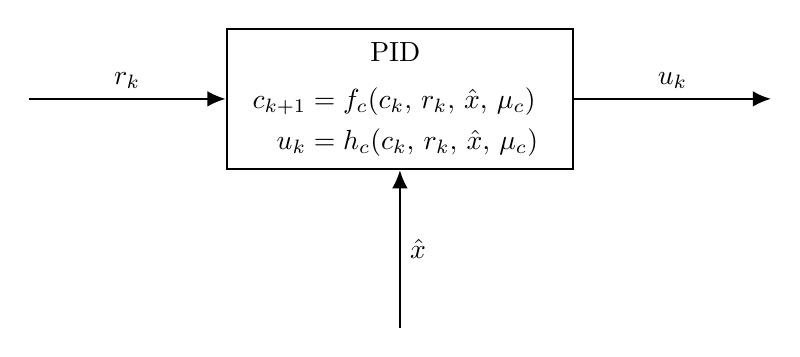
\begin{tikzpicture}[
  block/.style = {draw, thick, minimum height=3em, minimum width=6em, align=center},
  arrow/.style = {thick, -{Latex[width=2mm]}},
  node distance=2.5cm and 2.5cm
]

% PID Controller Block
\node[block] (siggen) {
  \begin{tabular}{c}
    PID \\[0.5em]
    $
    \begin{aligned}
      c_{k+1} &= f_c(c_k,\,r_k,\,\hat{x},\,\mu_c) \\
      u_k &= h_c(c_k,\,r_k,\,\hat{x},\,\mu_c)
    \end{aligned}
    $
  \end{tabular}
};

% Left input: r_k
\draw[arrow] ($(siggen.west)+(-2.5,0)$) -- 
  node[midway, above] {$r_k$} (siggen.west);

% Bottom input: \hat{x}
\draw[arrow] ($(siggen.south)+(0,-2.0)$) -- 
  node[midway, right] {$\hat{x}$} (siggen.south);

% Right output: u_k
\draw[arrow] (siggen.east) -- 
  node[midway, above] {$u_k$} ++(2.5,0);

\end{tikzpicture}
\end{document}
